\section{Investigación (CvLAC)}

El tercer y último capítulo aborda la dimensión más selectiva de la huella del egresado: la actividad científica registrada en el Currículum de Vida Laboral y Académica (CvLAC) de Minciencias. Al cruzar los documentos de la base de \num{174685} graduados de las seis sedes con los perfiles CvLAC se validan \textbf{\num{2535} perfiles de investigador}, asociados a \textbf{\num{3403} registros} de coincidencia nombre--documento. Esos \num{2535} perfiles se corresponden con \textbf{\num{2547} graduados} de la base ---algunos perfiles enlazan con más de un registro documental---, y son estos \num{2547} egresados, el \textbf{1,5\,\%} del total, los que entran al cruce multidimensional del informe. Es, con diferencia, la dimensión de menor cobertura: frente a los miles de contratistas del SECOP o de matrículas del RUES, aquí hablamos de un par de millares de personas. No es una limitación del cruce sino el reflejo de una realidad, pues la investigación formal con hoja de vida en Minciencias es una actividad minoritaria entre cualquier población de profesionales. Por eso este capítulo no pregunta cuántos investigan, sino quiénes son: su nivel de formación, su reconocimiento por Minciencias, qué producen, en qué área del conocimiento y desde qué carrera y sede lo hacen.

\subsection{Validación de las coincidencias}
A diferencia del SECOP y del RUES, donde el enlace se hace por documento de forma exacta, el cruce con CvLAC exige una validación adicional, porque la coincidencia de un nombre o de una cédula no basta para afirmar que el investigador es, en efecto, un graduado tomasino. La validación se apoya en dos clases de evidencia que vinculan el perfil con la Universidad. La primera es la formación: el perfil CvLAC declara entre sus títulos un programa cursado en la Universidad Santo Tomás, lo que confirma el paso del investigador por la institución. La segunda es el grupo: el perfil pertenece a un grupo de investigación adscrito a la Universidad, lo que documenta un vínculo institucional vigente aunque el título no aparezca registrado. Un perfil se valida cuando reúne al menos una de estas dos evidencias. Conviene leer la cifra de \num{2535} validados como un \emph{piso} y no como un techo, pues quedan fuera de ella los investigadores cuyo paso por la Universidad no quedó consignado ni en sus títulos ni en su afiliación a un grupo, y que el procedimiento, deliberadamente conservador, prefiere no contar antes que contar de más.

\subsection{Nivel de formación}
La Tabla~\ref{tab:cvlac_nivel} ofrece el primer retrato del investigador validado, y es un retrato de alta cualificación. El \textbf{68,6\,\%} de los \num{2535} investigadores ha alcanzado un nivel de posgrado: la maestría es el nivel más frecuente, con el 40,4\,\% de los validados, seguida del doctorado, con el 18,5\,\%, y de la especialización, con el 9,8\,\%; a ellos se suma un pequeño núcleo de cuatro posdoctorados. El pregrado como nivel máximo queda en el 19,3\,\% y un 12,0\,\% no consigna su nivel. El contraste con las otras dos dimensiones es nítido: mientras el contratista del SECOP o el comerciante del RUES pueden ejercer con el solo título profesional, el investigador con hoja de vida en Minciencias es, de manera característica, un egresado que prolongó su formación más allá del pregrado. La investigación se concentra en la cúspide de la trayectoria académica.

\begin{table}[H]\centering\footnotesize
\caption{Nivel máximo de formación de los graduados validados en CvLAC.}\label{tab:cvlac_nivel}
\begin{tabular}{lrr}
\toprule
\rowcolor{ustaazul}\textbf{\color{white}Nivel máximo de formación} & \textbf{\color{white}Investigadores} & \textbf{\color{white}\%} \\
\midrule
Maestría & 1.023 & 40,4\% \\
Pregrado & 488 & 19,3\% \\
Doctorado & 469 & 18,5\% \\
No identificado & 303 & 12,0\% \\
Especialización & 248 & 9,8\% \\
Posdoctorado & 4 & 0,2\% \\
\bottomrule
\end{tabular}
\end{table}

\subsection{Categoría Minciencias}
El alto nivel de formación no se traduce, sin embargo, en un reconocimiento equivalente por parte de Minciencias. La Tabla~\ref{tab:cvlac_categoria} muestra que solo \textbf{\num{288} de los \num{2535} investigadores validados} (el 11,4\,\%) ostentan una categoría vigente en la convocatoria de medición; los \num{2247} restantes ---el 88,6\,\%--- figuran sin categoría. Entre los categorizados, la distribución dibuja la pirámide esperable: la base la forman los \textbf{164 investigadores Junior}, por encima se sitúan los \textbf{91 Asociados} y en la cima los \textbf{31 Senior}, a los que se añaden dos Eméritos. Que dos de cada tres validados tengan posgrado pero solo uno de cada diez alcance categoría revela una brecha entre la cualificación formal y el reconocimiento del sistema nacional de ciencia, que exige una producción sostenida y certificada que la mayoría de los egresados ---investigadores ocasionales o en etapas tempranas--- todavía no acumula.

\begin{table}[H]\centering\footnotesize
\caption{Categoría de investigador (Minciencias) de los graduados validados.}\label{tab:cvlac_categoria}
\begin{tabular}{lrr}
\toprule
\rowcolor{ustaazul}\textbf{\color{white}Categoría Minciencias} & \textbf{\color{white}Investigadores} & \textbf{\color{white}\%} \\
\midrule
Sin categoría & 2.247 & 88,6\% \\
Investigador Junior (IJ) & 164 & 6,5\% \\
Investigador Asociado (I) & 91 & 3,6\% \\
Investigador Senior (IS) & 31 & 1,2\% \\
Investigador Emérito (IE) & 2 & 0,1\% \\
\bottomrule
\end{tabular}
\end{table}

\begin{figure}[H]\centering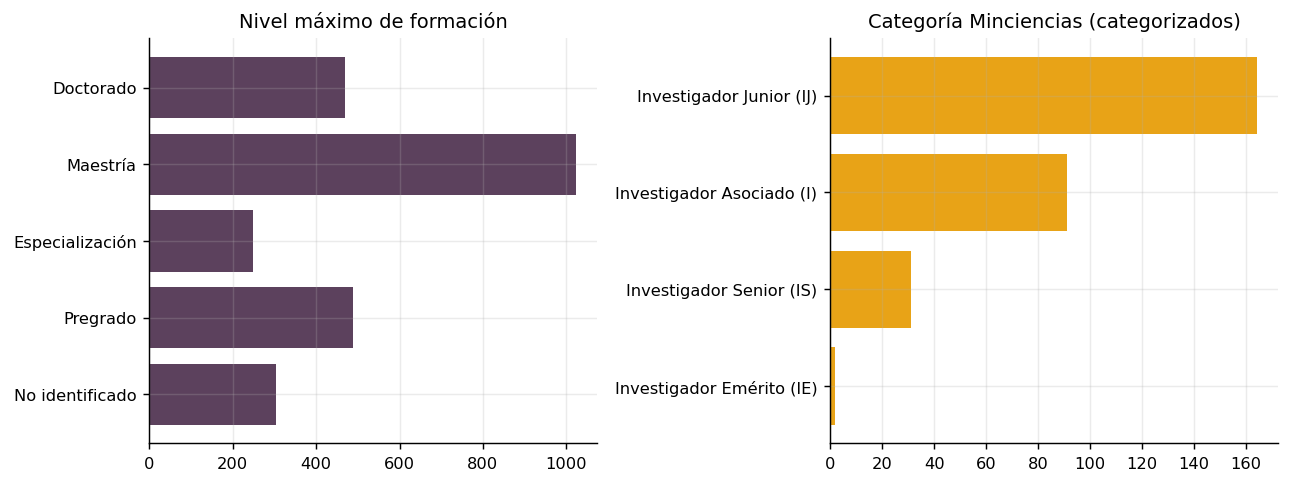
\includegraphics[width=0.90\linewidth]{figs_cruce/C1_cvlac_perfil.png}
\caption{Perfil del investigador validado: nivel máximo de formación y categoría Minciencias. El posgrado es mayoritario, pero la categorización es minoritaria.}\label{fig:cvlacperfil}\end{figure}

\subsection{Producción científica}
La Tabla~\ref{tab:cvlac_prod} agrega la producción declarada por los validados: \textbf{\num{13080} productos} registrados por los \num{2535} investigadores. La composición confirma una orientación marcadamente académica y, dentro de ella, la primacía indiscutida del \textbf{artículo}, que con \num{6434} productos concentra el 49,2\,\% de todo lo producido ---casi la mitad---. Le siguen los textos no científicos (18,5\,\%), los libros (10,1\,\%) y los capítulos de libro (6,9\,\%), de modo que la producción bibliográfica en sentido amplio domina por completo el panorama. Las formas de participación más aplicado ---consultorías, innovación de proceso, software--- aparecen en proporciones marginales, cada una por debajo del 2\,\%. El investigador tomasino produce, ante todo, conocimiento publicado en el formato canónico de la ciencia, y solo de manera residual transferencia tecnológica o productos de innovación.

\begin{table}[H]\centering\footnotesize
\caption{Producción científica de los graduados validados, por tipo de producto (CvLAC).}\label{tab:cvlac_prod}
\begin{tabular}{lrr}
\toprule
\rowcolor{ustaazul}\textbf{\color{white}Tipo de producto} & \textbf{\color{white}Productos} & \textbf{\color{white}\%} \\
\midrule
Artículos & 6.434 & 49,2\% \\
Textos no científicos & 2.422 & 18,5\% \\
Libros & 1.323 & 10,1\% \\
Capítulos de libro & 909 & 6,9\% \\
Demás trabajos & 497 & 3,8\% \\
Documentos de trabajo & 368 & 2,8\% \\
Otra prod. bibliográfica & 292 & 2,2\% \\
Consultorías & 264 & 2,0\% \\
Innovación de proceso & 164 & 1,3\% \\
Informes técnicos & 134 & 1,0\% \\
\bottomrule
\end{tabular}
\\[2pt]{\scriptsize\color{ustagris} Total de 13.080 productos registrados por los 2.535 investigadores validados.}
\end{table}

\begin{figure}[H]\centering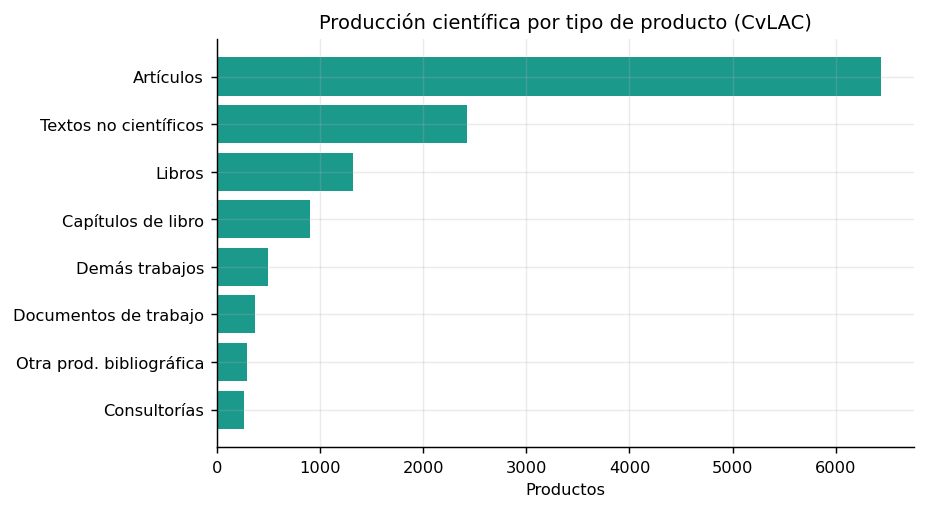
\includegraphics[width=0.74\linewidth]{figs_cruce/C2_cvlac_prod.png}
\caption{Producción científica de los graduados validados por tipo de producto. El artículo concentra cerca de la mitad de los \num{13080} productos.}\label{fig:cvlacprod}\end{figure}

\subsection{Categorización de las revistas}
La clasificación que declara CvLAC dice qué \emph{forma} tiene cada producto, pero no dónde se publica. Para caracterizar la calidad y el alcance de los artículos se extrajo el \textbf{ISSN} de cada uno ---\num{5640} menciones de revista en \num{1839} títulos distintos--- y se consultó cada revista en \textbf{OpenAlex}, el mayor catálogo bibliográfico abierto. El \textbf{82,5\,\%} de los artículos se publica en revistas indexadas en OpenAlex; de ellos, casi seis de cada diez (\textbf{59,5\,\%}) corresponden a revistas \textbf{colombianas} y un \textbf{55,1\,\%} a revistas de \textbf{acceso abierto} registradas en DOAJ (Tabla~\ref{tab:cvlac_revistas}). El perfil que emerge es el de una producción de visibilidad sobre todo nacional y de vocación abierta, con una presencia internacional minoritaria pero real ---tras Colombia aparecen Estados Unidos, España, Reino Unido y Brasil como países de edición---.

\begin{table}[H]\centering\footnotesize
\caption{Categorización de los artículos de los graduados según la revista (OpenAlex).}\label{tab:cvlac_revistas}
\begin{tabular}{lrr}
\toprule
\rowcolor{ustaazul}\textbf{\color{white}Indicador} & \textbf{\color{white}Artículos} & \textbf{\color{white}\%} \\
\midrule
Artículos con ISSN identificado & 5.640 &  \\
Revistas distintas (ISSN únicos) & 1.839 &  \\
En revista indexada en OpenAlex & 4.652 & 82,5\% \\
En revista de acceso abierto (DOAJ) & 2.561 & 55,1\% \\
En revista colombiana & 2.766 & 59,5\% \\
\bottomrule
\end{tabular}
\\[2pt]{\scriptsize\color{ustagris} ISSN extraído de cada artículo en CvLAC y consultado en OpenAlex.}
\end{table}

Clasificadas por el campo de conocimiento de la revista (Figura~\ref{fig:cvlaccampo}), las \textbf{Ciencias Sociales} concentran con holgura el grueso de los artículos, seguidas de la Economía y las Finanzas, las Ciencias de la Computación, las profesiones de la salud, las artes y humanidades, la medicina y la psicología. La distribución por campo de las revistas reproduce, desde la óptica editorial, el mapa disciplinar que ya mostraban las grandes áreas de actuación: la investigación de los graduados tomasinos es, ante todo, de ciencias sociales y humanas, con núcleos especializados en salud e ingeniería. Para una lectura de calidad en clave nacional, este mismo ISSN permitiría un cruce posterior con la categorización de \emph{Publindex} (A1, A2, B, C), que aquí queda planteado como extensión.

\begin{figure}[H]\centering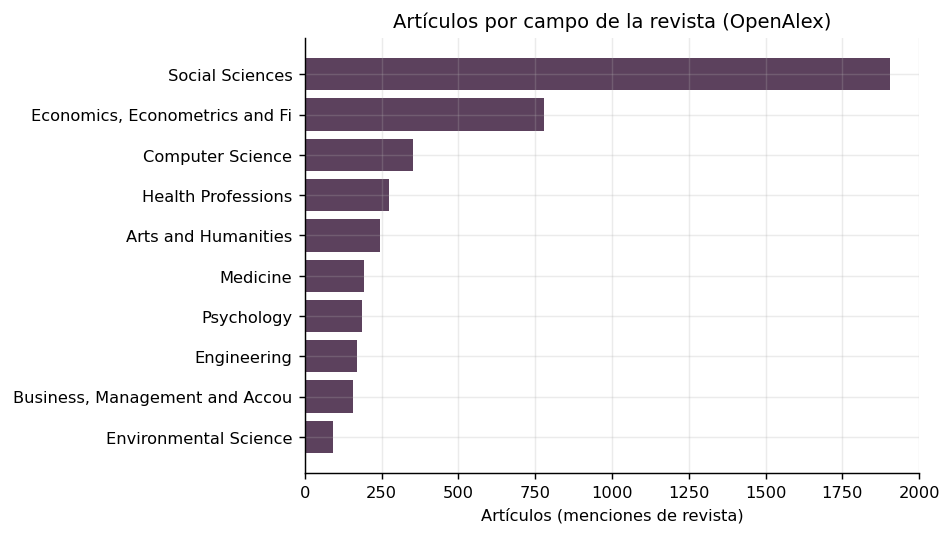
\includegraphics[width=0.74\linewidth]{figs_cruce/C4_cvlac_campo.png}
\caption{Artículos de los graduados validados según el campo de conocimiento de la revista (clasificación de OpenAlex).}\label{fig:cvlaccampo}\end{figure}

\subsection{Gran área de conocimiento}
Clasificando la producción de los investigadores por la gran área de conocimiento de Minciencias, el perfil global se inclina con claridad hacia las \textbf{Ciencias Sociales}, que reúnen \num{1345} investigadores ---más de la mitad del total---, seguidas a distancia por la \textbf{Ingeniería y Tecnología} (540) y las \textbf{Humanidades} (298); las Ciencias Médicas y de la Salud (166), las Ciencias Naturales (123) y las Ciencias Agrícolas (26) completan el cuadro. Más informativo que el agregado, sin embargo, es el cruce entre la carrera de origen y el área en que cada graduado investiga, que recoge la Figura~\ref{fig:cvlaccarreraarea}. Aquí se repite el patrón observado en el SECOP ---y que contrasta con la dispersión vista en el RUES---: cada carrera investiga en su área natural. El Derecho lo hace en Ciencias Sociales (el 93,6\,\% de sus investigadores), igual que la Economía (96,9\,\%) y la Psicología (92,1\,\%); las ingenierías se concentran en Ingeniería y Tecnología (el 99,1\,\% en Electrónica, el 86,7\,\% en Civil); la Cultura Física se vuelca a las Ciencias Médicas y de la Salud (76,9\,\%); y la Química Ambiental investiga, como cabe esperar, en Ciencias Naturales. La formación disciplinar de origen predice con notable fidelidad el territorio científico del egresado.

\begin{figure}[H]\centering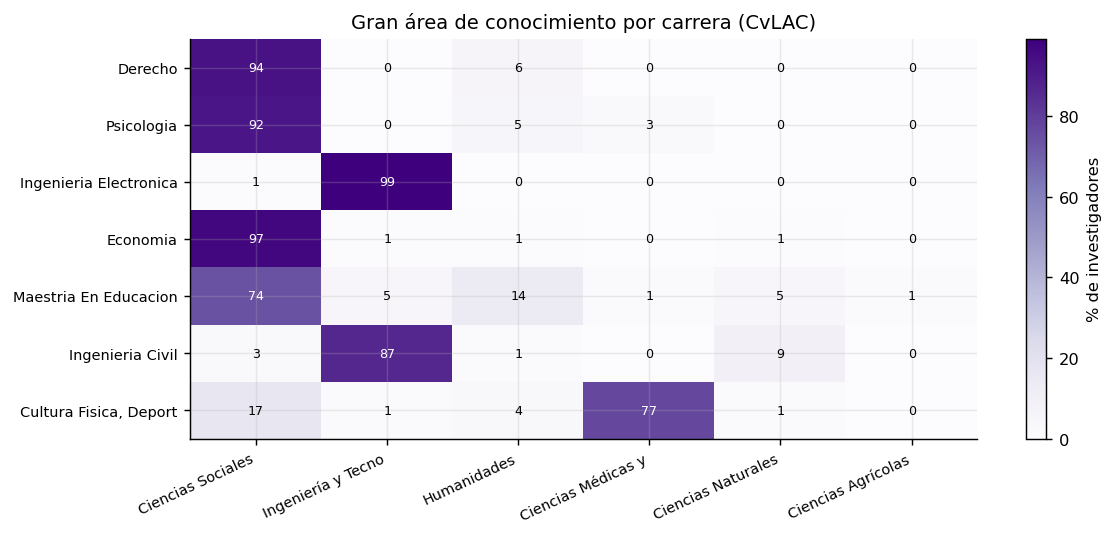
\includegraphics[width=0.92\linewidth]{figs_cruce/C3_cvlac_carrera_area.png}
\caption{Gran área de conocimiento de la investigación por carrera de origen (\% de investigadores por fila). Cada carrera investiga en su área natural.}\label{fig:cvlaccarreraarea}\end{figure}

\subsection{Investigación por carrera}
La Tabla~\ref{tab:cvlac_carrera} ordena los programas por número de graduados validados como investigadores y reproduce, en clave científica, jerarquías ya conocidas. El \textbf{Derecho} vuelve a encabezar, ahora con \textbf{273 investigadores}, una de las proporciones de doctorado más altas (24,1\,\%) y una mediana de dos productos por investigador. Le siguen la \textbf{Psicología} (115 investigadores), la \textbf{Ingeniería Electrónica} (113) y la \textbf{Economía} (99). Destaca la \textbf{Maestría en Educación}, que con 80 investigadores exhibe la mayor proporción de doctorado del cuadro (31,2\,\%) y la mediana de productos más alta (cuatro), un perfil coherente con un programa de posgrado orientado a la formación de investigadores. Más abajo aparecen las ingenierías Civil (78) y Ambiental (69), la Cultura Física (78), la Contaduría Pública (71), la Ingeniería de Telecomunicaciones (64), la Arquitectura (60) y los Negocios Internacionales (54). La investigación se reparte así entre las ciencias sociales, las ingenierías y, de forma destacada, los posgrados.

\begin{table}[H]\centering\footnotesize
\caption{Investigación por \textbf{carrera}: programas con más graduados validados en CvLAC.}\label{tab:cvlac_carrera}
\begin{tabular}{lrrr}
\toprule
\rowcolor{ustaazul}\textbf{\color{white}Programa (carrera)} & \textbf{\color{white}Investigadores} & \textbf{\color{white}\% doctorado} & \textbf{\color{white}Productos (mediana)} \\
\midrule
Derecho & 273 & 24,1\% & 2 \\
Psicologia & 115 & 13,0\% & 2 \\
Ingenieria Electronica & 113 & 8,0\% & 0 \\
Economia & 99 & 20,2\% & 1 \\
Maestria En Educacion & 80 & 31,2\% & 4 \\
Ingenieria Civil & 78 & 11,5\% & 0 \\
Cultura Fisica, Deporte Y Recr & 78 & 5,1\% & 0 \\
Contaduria Publica & 71 & 5,6\% & 0 \\
Ingenieria Ambiental & 69 & 1,4\% & 0 \\
Ingenieria De Telecomunicacion & 64 & 10,9\% & 0 \\
Arquitectura & 60 & 16,7\% & 2 \\
Negocios Internacionales & 54 & 0,0\% & 0 \\
\bottomrule
\end{tabular}
\\[2pt]{\scriptsize\color{ustagris} Programa de origen del graduado. Ordenado por nº de investigadores.}
\end{table}

\subsection{Investigación por sede}
La distribución de los investigadores validados por sede confirma la concentración esperable y la matiza con la densidad relativa. En números absolutos, \textbf{Bogotá} reúne \num{1434} investigadores ---más de la mitad---, seguida de Bucaramanga (528) y \textbf{Tunja} (388), y a distancia de Villavicencio (83), la VUAD (72) y Medellín (34). Bogotá y Tunja concentran, pues, el grueso de la actividad científica. Pero el número absoluto premia a las sedes de mayor tamaño y oculta la intensidad investigadora de las más pequeñas. Cuando los validados se ponen en relación con el volumen de graduados de cada sede, es \textbf{Tunja} la que muestra la mayor densidad relativa: produce proporcionalmente más investigadores que Bogotá pese a su menor tamaño. La sede de Boyacá emerge así no solo como la segunda en volumen, sino como la de vocación investigadora más intensa, un rasgo que el solo conteo absoluto dejaría invisible.

\subsection{Investigadores USTA fuera de la base de graduados}
El cruce con CvLAC arroja un hallazgo colateral que conviene registrar. Más allá de los \num{2535} perfiles validados como graduados, el ejercicio identifica \textbf{\num{3137} perfiles CvLAC adicionales con vínculo declarado a la Universidad Santo Tomás} ---por su formación, por su afiliación a un grupo de investigación o por ambas--- que no aparecen en la base de \num{174685} egresados. La explicación más probable es que se trate de docentes vinculados sin haberse graduado en la institución, de egresados de programas no incluidos en la base, o de graduados antiguos cuyo registro no quedó consignado en las fuentes disponibles. Sea cual sea su origen, este contingente de \num{3137} perfiles constituye un inventario valioso para futuros enlaces, pues señala la frontera entre la población medida en este informe y el universo más amplio de la comunidad investigadora tomasina.

\subsection{Síntesis del capítulo}
\begin{cajahallazgo}
La investigación es la dimensión más exigente y, a la vez, la mejor validada de la huella del egresado: solo \num{2535} graduados aparecen con hoja de vida en Minciencias, pero cada coincidencia se confirma por su formación o por su grupo en la Universidad. Es un colectivo de alta cualificación ---dos de cada tres tienen posgrado--- que, sin embargo, recibe poco reconocimiento formal del sistema nacional de ciencia, pues apenas uno de cada diez ostenta categoría Minciencias. Su producción se concentra en el formato canónico de la ciencia, con el artículo a la cabeza de los \num{13080} productos, y cada carrera investiga en su área natural: el Derecho y la Economía en ciencias sociales, las ingenierías en su campo técnico, la Química Ambiental en ciencias naturales. Bogotá y Tunja concentran la actividad, aunque Tunja despunta por su densidad investigadora. Y, como en las dimensiones anteriores, la cifra debe leerse como un piso y no como un techo, pues el procedimiento de validación, deliberadamente conservador, deja fuera a quien no dejó rastro de su paso por la Universidad.
\end{cajahallazgo}
